\documentclass[a4paper]{article}
\usepackage[left=1.0in, right=1.0in, top=1.0in, bottom=1in, includefoot, headheight=13.6pt]{geometry}
\usepackage{times}
\usepackage{tikz}
\usetikzlibrary{calc}
\parindent 0pt
\parskip 1.33ex

\title{BDI-Learning Discussion Paper:\\Understanding Stability}

\author{
Dhirendra Singh\\ 
dhirendra.singh@rmit.edu.au\\
}

\begin{document}
\maketitle

%% Section
\section{Background and Scope}

In this section we analyse the operation of the BUL scheme of \cite{Singh:AAMAS10} and highlight any nuances in it's operation. In particular we focus on the claim that BUL is able to learn well with applicability thresholds and show two cases where this claim fails. 


\section{Case 1: Stability without Success}

This example highlights the case where a plan $P$, that holds a solution for world $w$, may nonetheless become stable \textit{without} the solution being found. Consider the goal-plan hierarchy $T$ of Figure \ref{fig:t}. This is the structure where the BUL approach has a general advantage over ACL. Assume similar $k=3$ and $\epsilon=0.3$ values for stability calculation as used for the BUL specification in \cite{Singh:AAMAS10}.

\begin{figure}[ht]
\begin{center}
%!TEX root = ./dp5-stability.tex

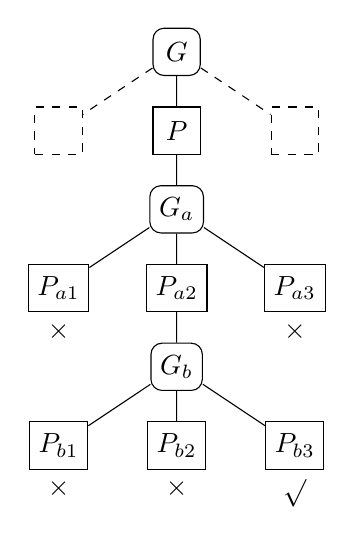
\begin{tikzpicture}[level distance=1.0cm]
\tikzstyle{succ}=[label=below:$\surd$]
\tikzstyle{fail}=[label=below:$\times$]
\tikzstyle{planbox}=[draw,minimum height=0.6cm,minimum width=0.6cm]
\tikzstyle{goalbox}=[draw,rounded corners,minimum height=0.6cm,minimum width=0.6cm]

\node[goalbox] {$G$}
	child[dashed] {node[planbox] {\phantom{$P$}}}
	child[solid] {node[planbox] {$P$}
		child {node[goalbox] (11) {$G_a$}
			child {node[planbox,fail] {$P_{a1}$}}
			child {node[planbox] {$P_{a2}$}
				child {node[goalbox] {$G_{b}$}
					child {node[planbox,fail] {$P_{b1}$}}
					child {node[planbox,fail] {$P_{b2}$}}
					child {node[planbox,succ] {$P_{b3}$}}
				}
			}
			child {node[planbox,fail] {$P_{a3}$}}
		}
	}
	child[dashed] {node[planbox] {\phantom{$P$}}}
;
\end{tikzpicture}



\end{center}
\caption{Goal-plan hierarchy $T$.}
\label{fig:t}
\end{figure}

Let us take up the analysis at the point where plan $P$ has been executed six times in the world $w$. The breakdown of the six executions is as follows: each of the three plans $P_{a*}$ has been executed twice and for each choice of $P_{a2}$, the plans $P_{b1}$ and $P_{b2}$ respectively were selected. As such, so far no plan has been deemed stable, and success has not been found. The executions are given by the traces below:

$\lambda1 = G[P:w] \cdot G_a[P_{a1}:w].$

$\lambda2 = G[P:w] \cdot G_a[P_{a2}:w] \cdot G_b[P_{b1}:w].$

$\lambda3 = G[P:w] \cdot G_a[P_{a3}:w].$

$\lambda4 = G[P:w] \cdot G_a[P_{a1}:w].$

$\lambda5 = G[P:w] \cdot G_a[P_{a2}:w] \cdot G_b[P_{b2}:w].$

$\lambda6 = G[P:w] \cdot G_a[P_{a3}:w].$

Up until now, the selection probabilities for the three $P_{a*}$ plans is the same and equal to $0.5$. In the seventh execution, let us assume $P_{a1}$ is selected, so that it now becomes stable and records the failure.

$\lambda7 = G[P:w] \cdot G_a[P_{a1}:w].$

The selection probabilities for the three $P_{a*}$ plans are now $[0.0,0.5,0.5]$ since the newly constructed decision tree of $P_{a1}$ predicts $p=0.0$ for $w$. Let us assume $P_{a2}$ is now selected at execution eight along with $P_{b1}$ below. 

$\lambda8 = G[P:w] \cdot G_a[P_{a2}:w] \cdot G_b[P_{b1}:w].$

On this failure $P_{b1}$ will not record as it is not stable. $P_{a2}$ that has had three execution in $w$ is now stable in it's own right --- but will also not record the failure since the choice of $P_{b1}$ below is not stable.


Finally, in the ninth execution, let's say $P_{a3}$ is selected, so that it now becomes stable and records the failure.

$\lambda9 = G[P:w] \cdot G_a[P_{a3}:w].$

After recording the failure in $P_{a3}$, the $RecordFailedTrace$ algorithm of \cite{Singh:AAMAS10} will now check to see if the failure should be propagated further up (in the trace $\lambda9$), i.e. should the failure be recorded for $P$, or, is goal $G_a$ stable for $w$. 

This is where it becomes interesting: $G_a$ turns out to be stable for $w$ because all it's plans are by now individually stable (i.e. satisfy the $k$ and $\epsilon$ requirements). $P_{a1}$ became stable at $\lambda7$, $P_{a2}$ at $\lambda8$, and $P_{a3}$ at $\lambda9$. As such, the failure is propagated up and $P$ records a failure.

The impact is that the predicted probability for $P_{a2}$ in $w$ drops from $0.5$ to $0.0$ and subsequently causes learning to fail where applicability thresholds are involved. 

This is a simple example to highlight the issue. The problem becomes more pronounced as we make $P_{a2}$ more ``complex''.



\section{Case 2: Stability and Multiple Worlds}

The second case highlights the disconnect between the fact that stability is a \textit{per world} concept whereas the decision tree spans \textit{multiple worlds}. So while stability ensures that the training set for a decision tree contains well-informed samples for some world, it says nothing about what this means for the use of this decision tree in other worlds.

Consider again the structure $T$ of Figure \ref{fig:t} and where we left off at $\lambda9$. The result was that $P_{a1}$ and $P_{a3}$ both had recorded a failure in $w$ while $P_{a2}$ has not yet recorded anything.

At this point let's say that $P$ is selected for a different world $w_1$. The resulting probabilities for $[P_{a1},P_{a2},P_{a3}]$ are now $[0.0,0.5,0.0]$ since the two decision trees built in $w$ will interpolate the failure result to $w_1$.

It is equally possible that $P_{a2}$ becomes stable with a recorded failure for yet another world $w_2$. If that were the case, then the resulting probabilities in $w_1$ would be $[0.0,0.0,0.0]$ due to interpolation. 

The impact is that the selection probabilities in $w_1$ may fall below the applicability threshold even when $w_1$ has never been witnessed before. As a result, once again the learning may fail.

%%%
\begin{thebibliography}{10}

\bibitem{Singh:AAMAS10}
D.~Singh, S.~Sardina, L.~Padgham, and S.~Airiau.
\newblock {Learning Context Conditions for BDI Plan Selection}.
\newblock In \emph{Proceedings of Autonomous Agents and Multi-Agent Systems
  (AAMAS)}, 2010.

\end{thebibliography}

\end{document}